%----------------------------------------------------------------------------------------
%	PACKAGES AND DOCUMENT CONFIGURATIONS
%----------------------------------------------------------------------------------------
% !TEX root=main.tex
\documentclass[10pt]{IEEEtran}

\usepackage[utf8]{inputenc}
\usepackage[english,spanish,activeacute]{babel}
\usepackage[cmex10]{amsmath}
\usepackage[numbers]{natbib}
\usepackage[acronym]{glossaries}
\usepackage{graphicx}
\usepackage{float}
\usepackage{xcolor}
\usepackage{listings}
\usepackage{xurl}
\usepackage{hyperref}
\hypersetup{
    colorlinks=true,
    linkcolor=blue,
    urlcolor=blue,
    citecolor=black
}


\definecolor{backcolour}{rgb}{1,1,1}
\definecolor{codegray}{rgb}{0.5,0.5,0.5}
\definecolor{codegreen}{rgb}{0,0.6,0}
\definecolor{codeyellow}{rgb}{1,0.7,0}
\definecolor{keywordscolour}{rgb}{0,0,1}

\lstdefinestyle{mystyle}{
    backgroundcolor=\color{backcolour},   
    commentstyle=\color{codegreen},
    keywordstyle=\color{keywordscolour},
    numberstyle=\tiny\color{codegreen},
    stringstyle=\color{violet},
    basicstyle=\ttfamily\footnotesize,
    breakatwhitespace=false,         
    breaklines=true,                 
    captionpos=b,                    
    keepspaces=true,                 
    numbers=left,                    
    numbersep=5pt,                  
    showspaces=false,                
    showstringspaces=false,
    showtabs=false,                  
    tabsize=2
}

\lstset{style=mystyle}


%----------------------------------------------------------------------------------------
% Acronyms
%----------------------------------------------------------------------------------------
\newacronym{pcr}{PCR}{Polymerase Chain Reaction}
\newacronym{tgf}{TGF}{Temperature Gradient Focusing}




\begin{document}

\newcommand{\titlepaper}{Least-Squares Filter Applied to a Temperature Control System using Simulink}

\title{\titlepaper}

\selectlanguage{english}
\author{\IEEEauthorblockN{Erick Andrés Obregón Fonseca}

\IEEEauthorblockA{erickof@estudiantec.cr}
\IEEEauthorblockA{\\MSc in Electronics -- Microelectronics Emphasis}
\IEEEauthorblockA{\\Instituto Tecnológico de Costa Rica}
}


\markboth{Obregón-Fonseca, \titlepaper}
{Shell \MakeLowercase{\textit{et al.}}: Bare Demo of IEEEtran.cls for Journals}


\IEEEtitleabstractindextext{%

\renewcommand{\abstractname}{Abstract}

\begin{abstract}
Accurate temperature monitoring is crucial in numerous daily and industrial applications. To address this, the utilization of a least-squares filter to effectively mitigate noise in the measured variable is explored in this paper.

For the study, a heating system was simulated using Simulink, incorporating Gaussian white noise into the output to mirror real-world disturbances. The system maintains a set-point of 25$^\circ$C, which represents the ambient temperature, and features an input pulse that activates the heating mechanism.

The findings indicate that the least-squares estimation technique successfully approximates the actual temperature with a high degree of accuracy, achieving results that closely match the true values.
\end{abstract}


\renewcommand{\IEEEkeywordsname}{Keywords}

\begin{IEEEkeywords}
Control System, Least Squares Filter, Matlab, Simulink, Temperature
\end{IEEEkeywords}}

\maketitle

\IEEEdisplaynontitleabstractindextext

\IEEEpeerreviewmaketitle

\selectlanguage{english}

\section{Introduction}

\subsection{Heating and Temperature Control}
Heating and temperature control systems have played a crucial role since the end of the 19th century. These systems have a wide range of applications from day-to-day tasks to industrial applications. \\

In 1895, Johnson made a significant breakthrough in temperature control with an automatic multi-zone temperature control system, designed to regulate the temperature in individual rooms or apartments~\cite{us542733s}. Subsequently, a variety of other applications have emerged. In the field of biotechnology, applications like~\acrfull{pcr}--such~\cite{MULLIS1987335, saiki1988, Bartlett2003, C6LC00984K, maltezos2010, mcknight2000, B208405H, hua2010multiplexed, mahjoob2008rapid, dinca2009fast, lien2009microfluidic, qiu2010large, hsieh2008enhancement, shen2005microchip, wang2009miniaturized}--and~\acrfull{tgf}~\cite{matsui2007temperature, ross2002microfluidic} for Electrophoresis requires tight temperature control~\cite{diagnostics3010033}. In biological science, precise temperature control is crucial, such as maintaining specific temperatures for cell viability or for~\acrshort{pcr} temperature cycling~\cite{diagnostics3010033, hung2005microfluid}. Also, in the food supply chain is important to ensure product quality and customer satisfaction, in transportation modes like sea, land, and railway, and in the logistic clusterization process can significantly reduce costs~\cite{baskutis2015temp}. On the other hand, in the automotive industry, thermal management in vehicle electrification enhances vehicle efficiency and battery performance~\cite{casals2016sustainability, previati2022thermal} and in specific areas like thermal management of lithium-ion batteries~\cite{karimi2013thermal}, electric machines~\cite{yang2017thermal}, and novel thermal management systems for batteries~\cite{al2018review}. \\

In critical applications such as mentioned before, accurate temperature monitoring is imperative. Consequently, the utilization of a least-squares filter to effectively mitigate noise in the target variable is explored.


\subsection{Least-Squares Filter}
Least-squares estimation theory was introduced by Gauss and further developed by Kalman, focusing on minimizing the sum of the squares of the difference between observed and estimated values~\cite{sorenson1970lse}. This methodology finds applications across a broad spectrum of categories, such as data curve fitting, parameter identification, and the realization of system models~\cite{crassidis2004dynamic}. This technique is versatile, with applications spanning various domains. Examples include calculating the damping properties of a fluid-filled damper based on temperature, identifying aircraft dynamic and static aerodynamic coefficients, determining orbit and attitude, locating position using triangulation, identifying modes of vibratory systems, and modern control strategies like some adaptive controllers where least-squares method is used to refine model parameters within the control system~\cite{crassidis2004dynamic}. \\

Assuming a set or a batch of measured values, $\tilde{y}_{j}$, of a process $y(t)$, taken at known discrete instants of time $t_{j}$:

\begin{equation}
    \left\{\tilde{y}_{1}, t_{1}; \tilde{y}_{2}, t_{2}; \ldots; \tilde{y}_{m}, t_{m}; \right\}
\end{equation}

and a proposed mathematical model of the form

\begin{equation}
    y(t) = \sum_{i = 1}^{n}{x_{i} h_{i}(t)},~~~m \geq n
\end{equation}

where

\begin{equation}
    h_{i}(t) \in \left\{ h_{1}(t), h_{2}(t), \ldots, h_{n}(t) \right\}
\end{equation}

are a set of independently specified basis functions where the measurements $\tilde{y}_{j}$ and the estimated output $\hat{y}_{j}$ can be related to the true and the estimated x-values leading to the Eq~\ref{eq:lse_w_error} and~\ref{eq:lse_wo_error}~\cite{crassidis2004dynamic}:

\begin{equation}
    \tilde{y}_{j} \equiv \tilde{y}(t_{j}) = \sum_{i = 1}^{n}{x_{i} h_{i}(t_{j}) + v_{j}},~~~j = 1, 2, \ldots, m
    \label{eq:lse_w_error}
\end{equation}

\begin{equation}
    \hat{y}_{j} \equiv \hat{y}(t_{j}) = \sum_{i = 1}^{n}{\hat{x}_{i} h_{i}(t_{j})},~~~j = 1, 2, \ldots, m
    \label{eq:lse_wo_error}
\end{equation}

where $v_{j}$ is the measurement error. This leads to the following identity:

\begin{equation}
    \tilde{y}_{j} = \sum_{i = 1}^{n}{\hat{x}_{i} h_{i}(t_{j}) + e_{j}},~~~j = 1, 2, \ldots, m
    \label{eq:lse_w_rerror}
\end{equation}

where residual error $e_{j}$ is defined by

\begin{equation}
    e_{j} \equiv \tilde{y}_{j} - \hat{y}_{j}
    \label{eq:residual_error}
\end{equation}

and this can be rewritten in compact matrix form as:

\begin{equation}
    \bf{\tilde{y}} = \bf{\it{H}} \bf{\hat{x}} + \bf{e}
\end{equation}

where ~\cite{crassidis2004dynamic} \\

$\bf{\tilde{y}} = \left[ \tilde{y}_{1} ~ \tilde{y}_{2} ~ \cdots ~ \tilde{y}_{m} \right] = $ measured y-values \\

$\bf{e} = \left[ e_{1} ~ e_{2} ~ \cdots ~ e_{m} \right] = $ residual errors \\

$\bf{\hat{x}} = \left[ \hat{x}_{1} ~ \hat{x}_{2} ~ \cdots ~ \hat{x}_{m} \right] = $ estimated x-values \\

In similar way, Eq~\ref{eq:lse_w_error_matrix} and~\ref{eq:lse_wo_error_matrix} can be represented using its compact matrix form as~\cite{crassidis2004dynamic}:

\begin{equation}
    \bf{\tilde{y}} = \bf{\it{H}} \bf{x} + \bf{v}
    \label{eq:lse_w_error_matrix}
\end{equation}

\begin{equation}
    \bf{\hat{y}} = \bf{\it{H}} \bf{\hat{x}}
    \label{eq:lse_wo_error_matrix}
\end{equation}

where \\

$\bf{x} = \left[ x_{1} ~ x_{2} ~ \cdots ~ x_{m} \right] = $ true x-values \\

$\bf{v} = \left[ v_{1} ~ v_{2} ~ \cdots ~ v_{m} \right] = $ measurements errors \\

$\bf{\hat{y}} = \left[ \hat{y}_{1} ~ \hat{y}_{2} ~ \cdots ~ \hat{y}_{m} \right] = $ estimated y-values \\

$\bf{\tilde{y}} = \left[ \tilde{y}_{1} ~ \tilde{y}_{2} ~ \cdots ~ \tilde{y}_{m} \right] = $ measured y-values \\

\subsubsection{Linear Least Squares}
The least squares principle selects particular $\hat{x}$ that minimizes the sum square of the residual errors as an optimum choice for the unknown parameters, given by~\cite{crassidis2004dynamic}:

\begin{equation}
    J = \frac{1}{2} e^{T} e
    \label{eq:lse}
\end{equation}

By substituting Eq~\ref{eq:lse_w_rerror} $e$ into the Eq~\ref{eq:lse}, applying the gradient of $\nabla_{\hat{x}} J$ and equaling to zero, the explicit solution for the optimal estimate is obtained:

\begin{equation}
    \bf{\hat{x}} = \left(\it{H}_{T} \it{H}\right)^{-1} \it{H}_{T} \bf{\tilde{y}}
\end{equation}


\subsubsection{Weighted Least Squares}
In cases where measurements are taken with varying degrees of precision, the approach of assigning equal weight appears to be logically flawed. To incorporate proper weighting, a least squares criterion of the form is established:

\begin{equation}
    J = \frac{1}{2} e^{T} \it{W} e
    \label{eq:wlse}
\end{equation}

producing the solution for $\hat{x}$ given by

\begin{equation}
    \bf{\hat{x}} = (\it{H}_{T} \it{W} \it{H})^{-1} \it{H}_{T} \hat{W} \bf{\tilde{y}}
\end{equation}

where $\it{W}$ is an $m \times m$ symmetric matrix~\cite{crassidis2004dynamic}. \\

When data is not available for batch processing--like in numerous real-world applications--but it is sequentially available, one might find it advantageous to calculate fresh estimates by considering all past measurements. For such cases, the covariance recursion form is used~\cite{crassidis2004dynamic}:

\begin{equation}
    \hat{x}(k + 1) = \hat{x}(k) + K(k + 1) \left[ \tilde{y}(k + 1) - H(k + 1) \hat{x}(k) \right]
    \label{eq:lse_recursion}
\end{equation}

where

\begin{equation}
    \begin{split}
        K(k + 1) = P(k) H^{t}(k + 1) [ H(k + 1) P(k) H^{T}(k + 1) +\\ W_{-1}(k + 1) ]^{-1}
    \end{split}
    \label{eq:lse_recursion_K}
\end{equation}

\begin{equation}
    P(k + 1) = \left[ I - K(k + 1) H(k + 1) \right] P(k)
    \label{eq:lse_recursion_P}
\end{equation}

with initial values of

\begin{equation}
    P(0) = \left[ \frac{1}{\alpha^{2}} I + H_{T}(0) W(0) H(0) \right]^{-1}
    \label{eq:lse_recursion_P0}
\end{equation}

\begin{equation}
    \hat{x}(0) = P(0) \left[ \frac{1}{\alpha} \beta + H_{T}(0) W(0) \hat{y}(0) \right]
    \label{eq:lse_recursion_x0}
\end{equation}


\subsection{System Model}
Given a basic heating house system that considers the outdoor and indoor temperature, the dynamics of the systems are described by a first-order differential equation with a time constant $\tau$~\cite{franklin1994dynsys}:

\begin{equation}
    \dot{T}(t) = \frac{1}{\tau} \left( T_{ambient} - T(t) \right) + \frac{K_{p}}{\tau} \cdot u(t)
\end{equation}

where

\begin{itemize}
    \item $\tau$ is the time constant of the system.

    \item $T_{ambient}$ is the temperature outside the house.

    \item $T(t)$ is the temperature in the house at time $t$.

    \item $K_{p}$ is the proportional gain or the heat rating of the system.

    \item $u(t)$ is the switch, $= 1$ if the system is on and $= 0$ if the system is off. \\
\end{itemize}

In the continuous-time state-space representation of a first-order system, the dynamics are described by the following first-order differential equation~\cite{ayomoh2012}:

\begin{equation}
    \dot{x} = a \cdot x(t) + b \cdot u(t)
\end{equation}

meaning that $a = 1/\tau$ and $b = K_{p}/\tau$. \\

For a first-order system with a continuous-time transfer function, the discrete-time representation can be obtained using methods such as Euler's method~\cite{griffiths2010}, backward difference~\cite{suleiman2011}, or Tustin's method~\cite{phillips1985}. The solution using Euler's methods is:

\begin{equation}
    y(k + 1) = \phi(k) y(k) + \Gamma(k) u(k)
    \label{eq:yk1}
\end{equation}

where

\begin{equation}
    \phi(k) = e^{a \cdot \Delta t}
    \label{eq:phi}
\end{equation}

\begin{equation}
    \Gamma(k) = \int_{0}^{\Delta t}{b} e^{a \cdot t} dt = \frac{b}{a} \left( e^{a \cdot \Delta t} - 1\right)
    \label{eq:gamma}
\end{equation}

and $\Delta t$ is the sampling time.

\section{Methodology}
The \acrshort{daq} system is implemented using an Arduino UNO R3 with a LM35 temperature sensor connected to it, as shown in Fig~\ref{fig:arduino_daq}.

\begin{figure}[H]
    \centering
    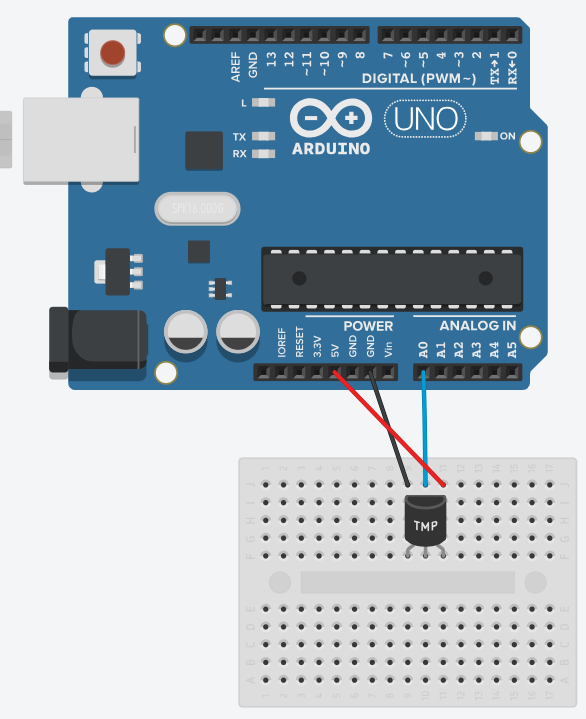
\includegraphics[width=0.6\linewidth]{figures/arduino_daq.png}
    \caption{Diagram representing the Arduino DAQ system}
~\label{fig:arduino_daq}
\end{figure}

The Arduino \acrshort{daq} system performs two primary functions. Initially, it measures the ambient temperature in millivolts ($mV$), which is then converted to Celcius degrees using a LM35.h library by Steven Wilmouth. The resulting temperature value is then supplied to the the Kalman filter algorithm. Secondly, it reads a digital signal indicating the status of the heating system, whether it is activate or deactivated that is used as the excitation function. \\

To take care of common matrix and vector mathematical operations like additon, substraction, multiplication, transposing, invertion and other, some miscelanious functions were coded, as shown below:

\lstinputlisting[language=C++]{codes/MathMatrix.hpp}

Kalman filter was implemented using Object-Oriented Programming. The class consists of three two main methods. For \textit{set\_params} method, constants like $H$, $R$, $\Gamma$, $\Phi$ and $Q$ are passed and are set as class attributes to use it later during prediction stage. The \textit{predict} method is used to apply the Kalamn algorithm. It takes the value of $x(k)$, $P(k)$, $y(t)$, and $u(k)$ to make the prediction of $x(k+1)$ and $P(k+1)$. The code can be seen below.

\lstinputlisting[language=C++]{codes/KalmanFilter.hpp}

Additionally, for the simulation, the following parameters are used:

\begin{itemize}
    \item $\tau$: the time constant of the system is set to 20s.

    \item $K_{p}$: the gain of the system is set to 0.5.

    \item $\sigma$: the standard deviation of the Gaussian white noise is set to 0.08.

    \item $\Delta t$: the sampling time is set to 1 seconds.
\end{itemize}

The parameters for the filter were computed as:

\begin{equation}
    R = \sigma^2 = (0.08)^2 = 0.0064
\end{equation}

\begin{equation}
    \phi(k) = e^{a \cdot \Delta t} = e^{-0.05 \cdot 1} = 0.6065
\end{equation}

\begin{equation}
    \Gamma(k) = \frac{0.025}{-0.05} \left( e^{-0.05 \cdot 1} - 1\right) = 0.1967
\end{equation}

The code used to test the Arduino \acrshort{daq} system, is shown below:

\lstinputlisting[language=C++]{codes/Daq.ino}



\section{Results and Discussion}

\section{Conclusions}


\bibliographystyle{IEEEtranN}
\bibliography{bibliography/bibliography}

\end{document}
